%!TEX program = xelatex
\documentclass[dvipsnames, svgnames,a4paper,11pt]{article}
% ----------------------------------------------------
%   中山大学物理与天文学院本科实验报告模板
%   作者:Huanyu Shi,2019级
%   知乎:https://www.zhihu.com/people/za-ran-zhu-fu-liu-xing
%   Github:https://github.com/huanyushi/SYSU-SPA-Labreport-Template
%   Last update : 2023.4.10
% ----------------------------------------------------

% ----------------------------------------------------- 
%	加边框的命令
%	参考:https://tex.stackexchange.com/questions/531559/how-to-add-the-page-border-for-first-two-pages-in-latex
\usepackage{tikz}
\usetikzlibrary{calc}
\usepackage{eso-pic}
\AddToShipoutPictureBG{%
\begin{tikzpicture}[overlay,remember picture]
\draw[line width=0.6pt] % 边框粗细
    ($ (current page.north west) + (0.6cm,-0.6cm) $)
    rectangle
    ($ (current page.south east) + (-0.6cm,0.6cm) $); % 边框位置
\end{tikzpicture}}


\usepackage{xcolor}
\definecolor{c1}{HTML}{2752C9} % 目录颜色
\definecolor{c2}{RGB}{190,20,83} % 引用颜色

\usepackage{ctex}
\usepackage[top=28mm,bottom=28mm,left=15mm,right=15mm]{geometry}
\usepackage{hyperref} 
\hypersetup{
	colorlinks,
	linktoc = section, % 超链接位置,选项有section, page, all
	linkcolor = c1, % linkcolor 目录颜色
	citecolor = c1  % citecolor 引用颜色
}
\usepackage{amsmath,enumerate,multirow,float}
\usepackage{tabularx}
\usepackage{tabu}
\usepackage{subfig}
\usepackage{fancyhdr}
\usepackage{graphicx}
\usepackage{wrapfig}  
\usepackage{physics}
\usepackage{appendix}
\usepackage{amsfonts}

%
\usepackage{tcolorbox}
\tcbuselibrary{skins,breakable}
\newtcolorbox{tbox}[2][]{
    colframe=black!70!,
    breakable,
    enhanced,
	boxrule =0.5pt,
    title = {#2},
    fonttitle = \large\kaishu\bfseries,
	drop fuzzy shadow,
    #1
}
\newtcolorbox[auto counter,number within=section]{question}[1][]{
  top=2pt,bottom=2pt,arc=1mm,
  boxrule=0.5pt,
%   frame hidden,
  breakable,
  enhanced, %跨页后不会显示下边框
  coltitle=c1!80!gray,
  colframe=c1,
  colback=c1!3!white,
  drop fuzzy shadow,
  title={思考题~\thetcbcounter:\quad},
  fonttitle=\bfseries,
  attach title to upper,
  #1
}

% ---------------------------------------------------------------------
%	利用cleveref改变引用格式,\cref是引用命令
\usepackage{cleveref}
\crefformat{figure}{#2{\textcolor{c2}{图 #1}}#3} % 图片的引用格式
\crefformat{equation}{#2{(\textcolor{c2}{#1})}#3} % 公式的引用格式
\crefformat{table}{#2{\textcolor{c2}{表 #1}}#3} % 表格的引用格式


% ---------------------------------------------------------------------
%	页眉页脚设置
\fancypagestyle{plain}{\pagestyle{fancy}}
\pagestyle{fancy}
\lhead{\kaishu 中山大学物理与天文学院基础物理实验\uppercase\expandafter{\romannumeral2}} % 左边页眉,学院 + 课程
\rhead{\kaishu  \quad 光学相差实验Ⅰ} % 右边页眉,实验报告标题
\cfoot{\thepage} % 页脚,中间添加页码


% ---------------------------------------------------------------------
%	对目录、章节标题的设置
\renewcommand{\contentsname}{\centerline{\huge 目录}}
\usepackage{titlesec}
\usepackage{titletoc}
% \titleformat{章节}[形状]{格式}{标题序号}{序号与标题间距}{标题前命令}[标题后命令]
\titleformat{\section}{\centering\LARGE\songti}{}{1em}{}

% ---------------------------------------------------------------------
%   listing代码环境设置
\usepackage{listings}
\lstloadlanguages{python}
\lstdefinestyle{pythonstyle}{
backgroundcolor=\color{gray!5},
language=python,
frameround=tftt,
frame=shadowbox, 
keepspaces=true,
breaklines,
columns=spaceflexible,                   
basicstyle=\ttfamily\small, % 基本文本设置,字体为teletype,大小为scriptsize
keywordstyle=[1]\color{c1}\bfseries, 
keywordstyle=[2]\color{Red!70!black},   
stringstyle=\color{Purple},       
showstringspaces=false,
commentstyle=\ttfamily\scriptsize\color{green!40!black},%注释文本设置,字体为sf,大小为smaller
tabsize=2,
morekeywords={as},
morekeywords=[2]{np, plt, sp},
numbers=left, % 代码行数
numberstyle=\it\tiny\color{gray}, % 代码行数的数字字体设置
stepnumber=1,
rulesepcolor=\color{gray!30!white}
}




% ---------------------------------------------------------------------
%	其他设置
\def\degree{${}^{\circ}$} % 角度
\graphicspath{{./images/}} % 插入图片的相对路径
\allowdisplaybreaks[4]  %允许公式跨页 % 导入模板的相关设置
\usepackage{lipsum}
\usepackage{enumitem}
\setlist[enumerate]{label=\textup{(\arabic*)}}



%---------------------------------------------------------------------
%	正文
%---------------------------------------------------------------------

\begin{document}


\begin{table}
	\renewcommand\arraystretch{1.7}
	\begin{tabularx}{\textwidth}{
		|X|X|X|X
		|X|X|X|X|}
	\hline
	\multicolumn{2}{|c|}{预习报告}&\multicolumn{2}{|c|}{实验记录}&\multicolumn{2}{|c|}{分析讨论}&\multicolumn{2}{|c|}{总成绩}\\
	\hline
	\LARGE25 & & \LARGE30 & & \LARGE25 & & \LARGE80 & \\
	\hline
	\end{tabularx}
\end{table}


\begin{table}
	\renewcommand\arraystretch{1.7}
	\begin{tabularx}{\textwidth}{|X|X|X|X|}
	\hline
	专业:& 物理学 &年级:& 2022级\\
	\hline
	姓名:& 戴鹏辉  & 学号: & 2344016 \\
	\hline
	日期:& 2024/03/11 & 教师签名:& \\
	\hline
	\end{tabularx}
\end{table}

\begin{center}
	\LARGE CB1+ \quad 迈克尔逊干涉及应用(白光干涉) 
\end{center}

\textbf{【实验报告注意事项】}
\begin{enumerate}
	\item 实验报告由三部分组成:
		\begin{enumerate}
			\item 预习报告:(提前一周)认真研读\underline{\textbf{实验讲义}},弄清实验原理;实验所需的仪器设备、用具及其使用(强烈建议到实验室预习),完成课前预习思考题;了解实验需要测量的物理量,并根据要求提前准备实验记录表格(第一循环实验已由教师提供模板,可以打印)。预习成绩低于10分(共20分)者不能做实验。
		    \item 实验记录:认真、客观记录实验条件、实验过程中的现象以及数据。实验记录请用珠笔或者钢笔书写并签名(\textcolor{red}{\textbf{用铅笔记录的被认为无效}})。\textcolor{red}{\textbf{保持原始记录,包括写错删除部分,如因误记需要修改记录,必须按规范修改。}}(不得输入电脑打印,但可扫描手记后打印扫描件);离开前请实验教师检查记录并签名。
		    \item 分析讨论:处理实验原始数据(学习仪器使用类型的实验除外),对数据的可靠性和合理性进行分析;按规范呈现数据和结果(图、表),包括数据、图表按顺序编号及其引用;分析物理现象(含回答实验思考题,写出问题思考过程,必要时按规范引用数据);最后得出结论。
		\end{enumerate}
	\textbf{实验报告就是将预习报告、实验记录、和数据处理与分析合起来,加上本页封面。}
	
	\item 每次完成实验后的一周内交\textbf{实验报告}(特殊情况不能超过两周)。
	
	\item 除实验记录外,实验报告其他部分建议双面打印。
\end{enumerate}
\textbf{【安全注意事项】}
	\begin{enumerate}
		\item 实验过程中,光源不要随意打开关闭;
		\item 严禁用手触光学镜头的表面;
		\item 严禁用强力和斜向力旋转测微头,这样会损坏测微头或其他部件;
		\item 不要拆卸传动机构,以免影响仪器正常使用;
		\item 实验过程中,数条纹时,避免桌面的振动。
	\end{enumerate}

\clearpage
\tableofcontents
\clearpage

\setcounter{section}{0}
\section{CB1+ \quad 迈克尔逊干涉及应用(白光干涉) \quad\heiti 预习报告}
	
\subsection{实验目的}
\begin{enumerate}
	\item 观察等倾、等厚干涉现象及调节白光干涉条纹;
	\item 学习用迈克尔逊干涉仪测量钠光谱波长差的方法;
	\item 学习用白光干涉测量透明薄片折射率的方法;
	\item 用迈克尔逊干涉仪测量多种光源的相干长度;
	
\end{enumerate}

\subsection{仪器用具}
	\begin{table}[htbp]
		\centering
		\renewcommand\arraystretch{1.6}
		% \setlength{\tabcolsep}{10mm}
		\begin{tabular}{p{0.05\textwidth}|p{0.20\textwidth}|p{0.05\textwidth}|p{0.5\textwidth}}
			\hline
			编号& 仪器用具名称 & 数量 &  主要参数(型号,测量范围,测量精度等) \\
			\hline
			1& 精密干涉仪 & 1 & SGM-3 \\
			
			2& He-Ne 激光器 & 1 & -- \\
			
			3& 钠钨双灯 & 1 & -- \\
			
			4& 汞灯 & 1 & -- \\
			
			5& 透明薄片 & 1 & -- \\
			
			6& 螺旋测微计 & 1 & -- \\
			\hline
		\end{tabular}
	\end{table}

\subsection{原理概述}
	
	\begin{enumerate}
		\item \textbf{测钠双黄线的波长差}
			
			钠黄光含有两种波长相近的光($\lambda_1 = 589.0 nm$, $\lambda_2 = 589.6 nm$)。 采用钠灯作光源时, 两条谱线形成各自的干涉条纹,在视场中的两套干涉条纹相互叠加。由于波长不同,同级条纹之间会产生错位($\lambda_1$的某一级的暗条纹可能会和 $\lambda_2$的另一级的亮条纹重合)。 在移动反射镜$M_1$ (光程差发生变化) 过程中,干涉条纹会出现清晰与模糊的周期性变化,称为“光拍现象”。 其原理如下。\\
			
			设两条光路的光程差$L=2d$,由光的干涉条件可知:当 $L = k_1 \lambda_1$($k_1$ 为整数)时,在视场$E$中心处干涉加强; 当$L=(k_2+\frac{1}{2})\lambda_2$($k_2$为整数)时,在视场$E$ 中心处干涉减弱。\\
			
			视场$E$中心处$\lambda_1$和$\lambda_2$两种单色光干涉条纹相互叠加。若逐渐增大 $M_1$与$ M_2 $的间距 $d$,当$\lambda_1$的第$ k_1$级亮条纹和$\lambda_2$的第 $ k_2$级暗条纹相重合时,叠加而成的干涉条纹清晰度最低,此时干涉条纹出现第一次模糊,记录此时的光程差为 $L_A$. \\     %有
			
	%		\[ L_A=k_1\lambda_1=(k_2+\frac{1}{2})\lambda_2 \]
			
			若继续增大$M_1$与$ M_2 $的间距,使得视场$ E $中心处的光程差增加至$ L_B$, 此时$\lambda_1$的第$(k_1+n)$级亮条纹和$\lambda_2$的第$(k_2+n)$级亮条纹相重合,叠加而成的干涉条纹亮度最高,此时干涉条纹恢复清晰。\\
			
			继续增大$M_1$与$M_2$的间距, 使得视场 $E$ 中心处的光程差增加至 $L_C$, 此时 $\lambda_1$的第$(k_1+m)$ 级亮条纹和$\lambda_2$ 的第$ (k_2 + m - 1) $级暗条纹相重合时,叠加而成的干涉条纹清晰度再次出现最低,此时干涉条纹出现第二次模糊,记录此时的光程差为 $L_C$ .\\
			
			设干涉条纹出现一次模糊→清晰→模糊的变化时, 反射镜$ M_1 $的移动距离为$\Delta d$,则$A $处和$ C $处前后的光程差变化为$\Delta L_{AC}=L_C-L_A=2\Delta d=m\lambda_1=(m-1)\lambda_2$,则$\Delta \lambda=\lambda_2-\lambda_1=\lambda_2/m$,$m=2\Delta d/\lambda_1$,得到最后结果为:
			\[ \Delta \lambda\equiv\lambda_2-\lambda_1=\frac{\lambda_1\lambda_2}{2\Delta d}=\frac{\bar{\lambda}^2}{2\Delta d} 
			\]
			记录下干涉条纹出现一次“模糊→清晰→模糊” 的变化时, 反射镜$ M_1 $移动的距离$\Delta d$, 结合钠双黄线的平均波长 ,即可利用上式求得钠双黄线的波长差。\\
			
			\begin{figure}[htbp]
				\centering
				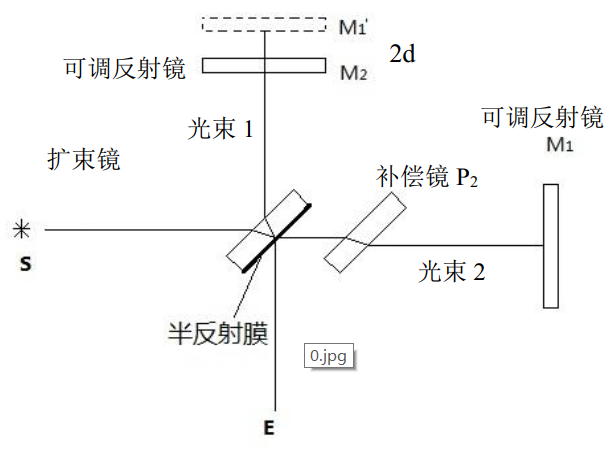
\includegraphics[width=0.5\textwidth]{graph1.png}
				\caption{迈克尔逊干涉仪光路图}
				\label{fig:fig1}
			\end{figure}
			
			
		\item \textbf{白光干涉的调节,并测定透明薄片的厚度 $t$ 或者折射率 $n$}
		
%			在迈克尔逊干涉实验中,先采用激光光源(安装上扩束镜),调节出定域等倾干涉圆环。再调节可移动反射镜$ M_2 $的预置测微头,减小两干涉臂的光程差$ L$(此过程中干涉圆环不断内缩,在观察屏中心$E$处不断“消失”),直至观察屏上只剩下几个较粗的干涉圆环(或圆环几乎消失)。这时候意味着两干涉臂的光程差$L$近似等于零。这时候撤掉扩束镜, 换上扩散的汞灯光源(毛玻璃),把观察屏翻到背后有玻璃的一面,然后微调可调反射镜 $M_2$ 背面的三个螺钉(调节$ M_2 $的倾斜度),此时应能在玻璃镜(视场)中观察到域等倾干涉圆环。再调节可移动反射镜 $M_2$ 的预置测微头,减小两干涉臂的光程差$L$(此过程中干涉圆环不断内缩,在观察屏中心$E$ 处不断“消失”),直至观察屏上只剩下非常粗大的干涉圆环。换上扩散的白光光源(本实验中采用溴钨灯加毛玻璃代替), 微调$ M_1$ 精密测微头, 此时应能在玻璃镜(视场) 中观察到彩色的条纹,此即为“白光等厚干涉条纹”。 在视场中心处的彩色条纹之间还可观察到一条全黑的条纹,称为“中心暗纹”。\\
%			
%			然后在反射镜 $M_1$ 与分束镜 $P_1$之间放上折射率为 $n$,厚度为 $t$ 的透明薄片,且尽量使薄片与$ M_1 $镜平行,则此时两干涉臂的光程差要比原来增大
%			\[ 
%			\Delta L=2t(n-1) 
%			\]
%			放上透明薄片后,透过观察屏玻璃观察透明薄片处,可以看到视场中的白光干涉彩色条纹消失。此时如果将反射镜$ M_1 $镜向前朝分束镜 $P_1$方向移动一段距离$\Delta d$, 使得$\Delta d = \Delta L /2$,则白光彩色干涉条纹重新出现。此时有
%			\[ 
%			\Delta d=t(n-1) 
%			\]
%			测出$ M_1 $镜的移动量$\Delta d$, 若已知透明薄片的厚度$ t$, 则可由上式可求出透明薄片的折射率$n$;反之,若已知透明薄片的折射率$n$,可求出透明薄片的厚度$t$。
		
			迈克尔逊干涉实验的变形实验中,首先使用激光光源和扩束镜调节出定域等倾干涉圆环,表示两干涉臂的光程差接近零。接着,换上扩散的汞灯光源,在观察屏翻到背后有玻璃的一面,微调可调反射镜 $M_2$ 的倾斜度,调节干涉条纹直至只剩下非常粗大的干涉圆环。然后,换上扩散的白光光源,微调$ M_1$ 的精密测微头,在玻璃镜(视场)中观察到彩色的条纹,称为“白光等厚干涉条纹”。接着,在反射镜 $M_1$ 与分束镜 $P_1$ 之间放上折射率为 $n$,厚度为 $t$ 的透明薄片,两干涉臂的光程差增大为 $\Delta L=2t(n-1)$,透过观察屏玻璃观察透明薄片处,可以看到视场中的白光干涉彩色条纹消失。最后,将反射镜$ M_1 $向前朝分束镜 $P_1$ 方向移动一段距离$\Delta d$,使得$\Delta d = \Delta L /2$,此时白光彩色干涉条纹重新出现。通过测量$ M_1 $镜的移动量$\Delta d$,可以根据$\Delta d=t(n-1)$计算出透明薄片的折射率$n$或厚度$t$。
			
	\end{enumerate}

	




\subsection{实验前思考题}

	\begin{question}
		如何测量透明溶液的折射率?请自行就相关实验原理进行调研,并设计合理试验方案。
	\end{question}
		可以使用迈克尔逊干涉仪测量透明溶液的折射率,方法简述如下:
		
		\begin{enumerate}
			\item 准备设备:设置迈克尔逊干涉仪,确保所有光学元件清洁并正确对准。
			\item 校准干涉仪:在不放入样品的情况下,调整干涉仪直至观察到清晰的干涉条纹。
			\item 放置样品:将装有透明溶液的比色皿放置在干涉仪的一臂中,确保比色皿平行于光束。
			\item 观察条纹变化:开启干涉仪,观察由于溶液折射率不同而引起的干涉条纹移动。
			\item 数据记录:记录条纹移动的数量,这与溶液的光程差有关。
			\item 计算折射率:使用公式 $n=1+\frac{\lambda}{2d}$
			
			   其中$n$是折射率,$\lambda$是光的波长,$ d$是比色皿的厚度,$m$是条纹移动的数量。
		\end{enumerate}
		
		测量折射率的方法还有多种,除了迈克尔逊干涉仪法外,还包括:
		
		\begin{itemize}
			\item 几何光学方法:利用斯涅尔定律,可以通过最小偏向角法或极限角法来测量折射率。这些方法通常需要一个透明的三棱镜样品。
			\item 波动光学方法:通过光程差和干涉现象来测量折射率,例如使用马赫干涉仪或法布里珀罗干涉仪
			\item 分光光度法:这种方法通过测量样品的反射率和透射率来计算折射率。它可以进一步细分为菲涅耳公式法、布儒斯特定律法和接近垂直入射时的反射法。
			\item 椭圆偏振测量法:这种方法通过测量反射光的振幅比和相移来直接测量折射率,需要针对每种材料的特定光学模型。
			\item ATR法:采用全反射原理,利用样品与棱镜的接触面发生反射,反射角与入射角之差与样品折射率之间存在固定的关系,从而计算出样品的折射率。
			\item 位移法:通过比较两种介质中一个光点的位置变化,计算出样品的折射率。具体方法包括折射平台法、折射浸渍法等。
		\end{itemize}
		每种方法都有其适用的情况和限制,选择合适的方法取决于样品的性质和实验条件。
		

	\begin{question}
		如何测量汞灯光源的相干长度?请自行就相关实验原理进行调研,并设计具体实验方案。
	\end{question}
		
		可以使用迈克尔逊干涉仪测量汞灯光源的相干长度,具体实验步骤如下:
		\begin{enumerate}
			\item 调整激光器:打开He-Ne激光器,调出清晰的等倾非定域干涉条纹。调节动镜M2的镜面调节螺丝,使观察屏上出现清晰的干涉条纹。
			\item 汞灯光源的安装:撤掉激光器,换上低压汞灯光源。在汞灯光源与平面反射镜间放置毛玻璃,观察是否有直线条纹出现。
			\item 观察干涉条纹:从E点位置用单眼观察M2的位置,检查是否有黑白相间的直线条纹。如果没有出现,则适当调节M2的镜面调节螺丝,直至视野中出现直线条纹。
			\item 测量相干长度:向同一方向转动M2的微调鼓轮,使视野中的彩色直线条纹变弯曲。在条纹刚刚变弯曲的时刻,记下M2微调鼓轮的初始读数d1和彩色直线条纹刚刚变弯曲时读数d2。相干长度即为$d=\frac{1}{2}(d_1-d_2)$
		\end{enumerate}
		

\clearpage
\begin{table}
	\renewcommand\arraystretch{1.7}
	\centering
	\begin{tabularx}{\textwidth}{|X|X|X|X|}
	\hline
	专业:& 物理学 &年级:& 2022级 \\
	\hline
	姓名:& 戴鹏辉 & 学号:& 22344016 \\
	\hline
	室温:& 26℃ & 实验地点: & A505 \\
	\hline
	学生签名:& & 评分: &\\
	\hline
	实验时间:& 2024/03/14 & 教师签名:&\\
	\hline
	\end{tabularx}
\end{table}

\section{CB1+ \quad 迈克尔逊干涉及应用(白光干涉) \quad\heiti 实验记录}
\subsection{实验内容和步骤}

	\subsubsection{实验一 测钠双黄线的波长差}
	
		\begin{enumerate}
			\item 首先调节迈克尔逊干涉仪, 使产生定域等倾干涉条纹:
			
				\begin{enumerate}[label=\roman*.]
					\item 安装并打开 $He-Ne$ 激光器(注意不要直射眼睛), 但先不安装扩束镜, 使激光束从分束镜$ P_1$的中心附近入射;
					
					\item 调节可调反射镜 $M_2$ 背面的三个螺钉,使得 $M_1$ 和 $M_2$ 反射的光点的最亮处在观察屏 $E$ 上重合;
					
					
					\item 装上扩束镜(以获得点光源),此时应能在观察屏上看到等倾干涉条纹(如观察不到,则可微调固定激光器的螺钉,使得光束能顺利通过扩束镜)。
				\end{enumerate}
				
				\begin{figure}[htbp]
					\centering
					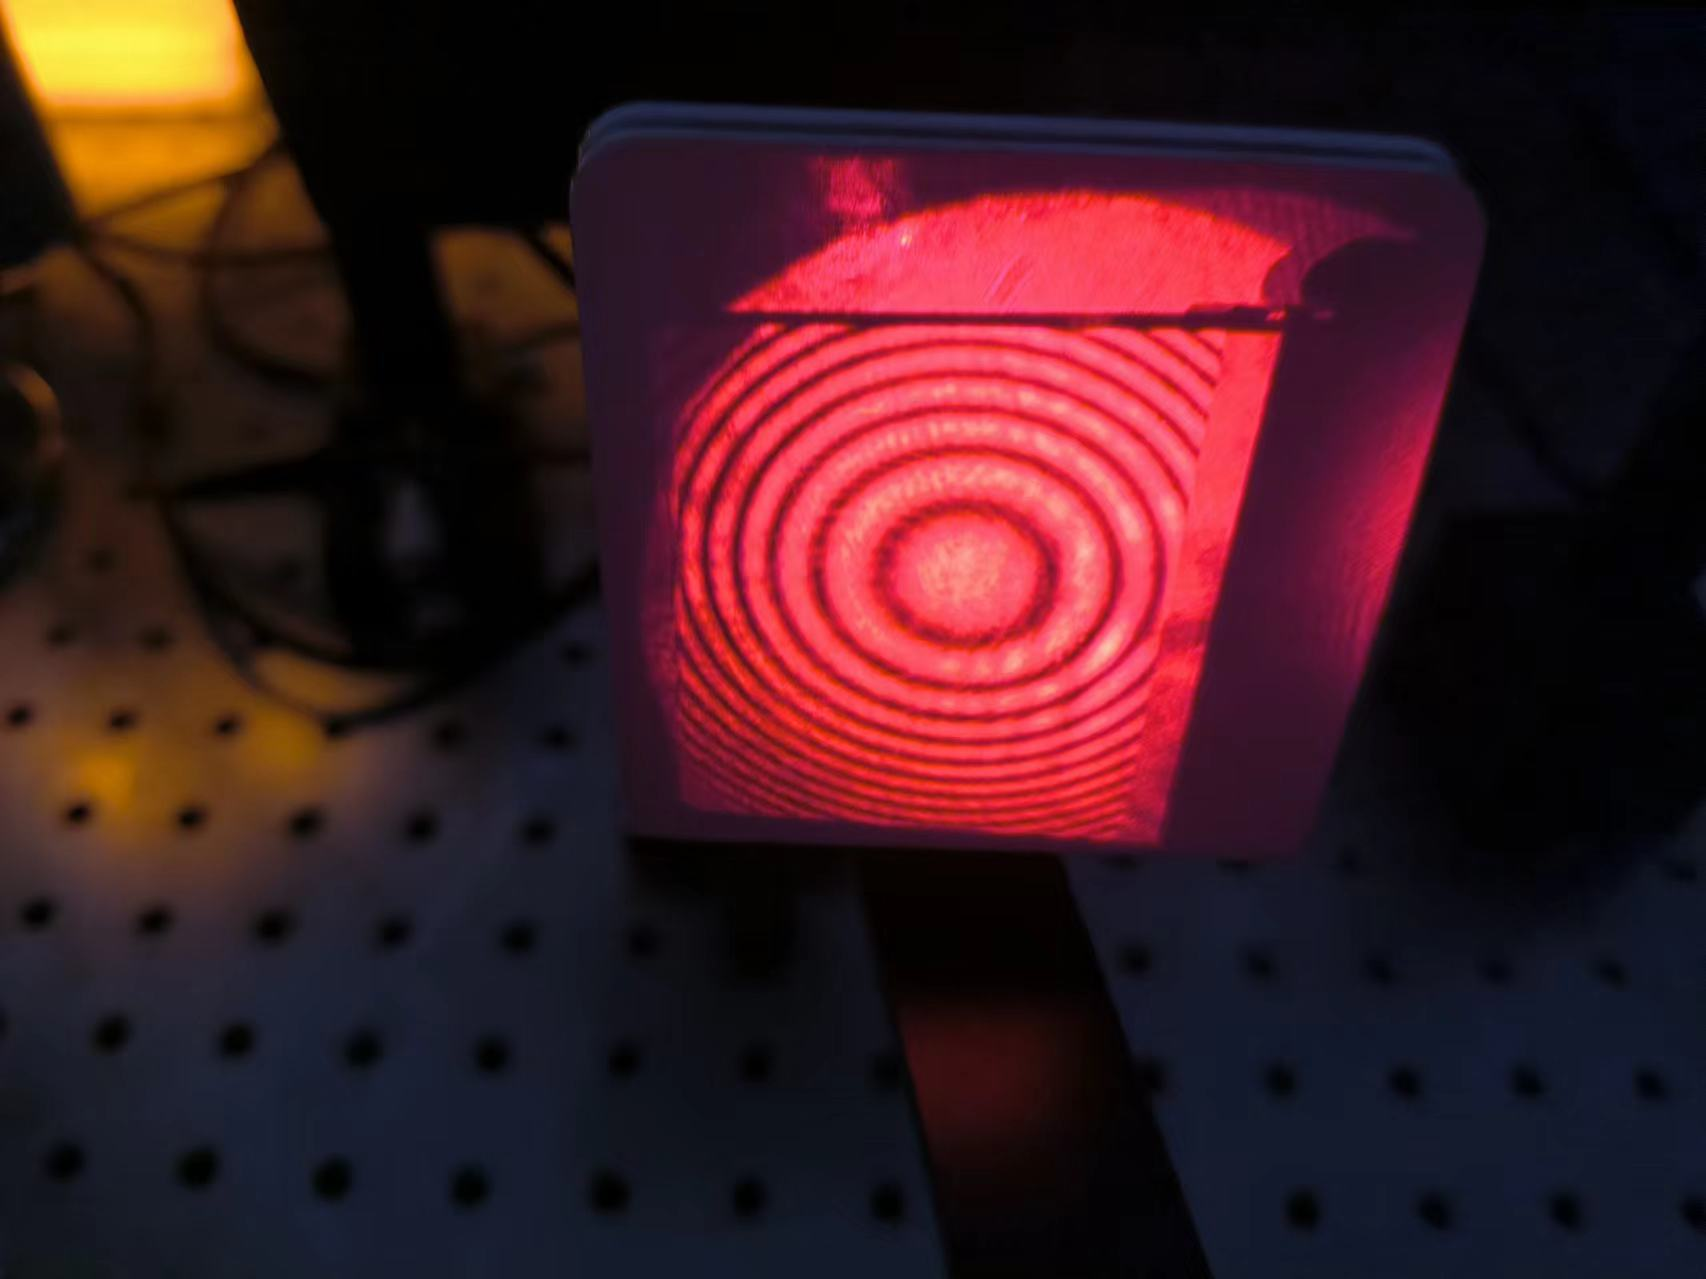
\includegraphics[width=0.7\textwidth]{graph2.jpg}
					\caption{激光光源的干涉图像}
					\label{fig:graph2}
				\end{figure}
			
			\item 然后调节可移动反射镜 $M_1$ 的精密测微头,减小两干涉臂的光程差 $L$,直至观察屏上只剩下几个较粗的干涉圆环或圆环几乎消失,这时候两干涉臂的光程几乎相等,光程差近似等于零。
			
			\item 不安装扩束镜。改用钠灯,灯前装有毛玻璃使光散射。观察屏改为平面玻璃反射镜;
			
			\item 从观察屏的玻璃中观察,仔细调节 M2 镜后的三颗倾斜度调节螺钉和 $M_1$镜的位置,可观察到黄黑相间的直线状的等厚干涉条纹;
			
			\item 调节精密测微头,移动反射镜 $M_1$,观察条纹“模糊→清晰→模糊” 的周期变化过程,记录每一次干涉条纹“模糊”时候精密测微头的读数,随后计算出$M_1$ 镜移动的距离$\Delta d$,即可根据公式计算钠双黄线的波长差$\Delta \lambda\equiv\lambda_2-\lambda_1=\frac{\lambda_1\lambda_2}{2\Delta d}=\frac{\bar{\lambda}^2}{2\Delta d} $

		\end{enumerate}
		
		\begin{figure}[htbp]
			\centering
			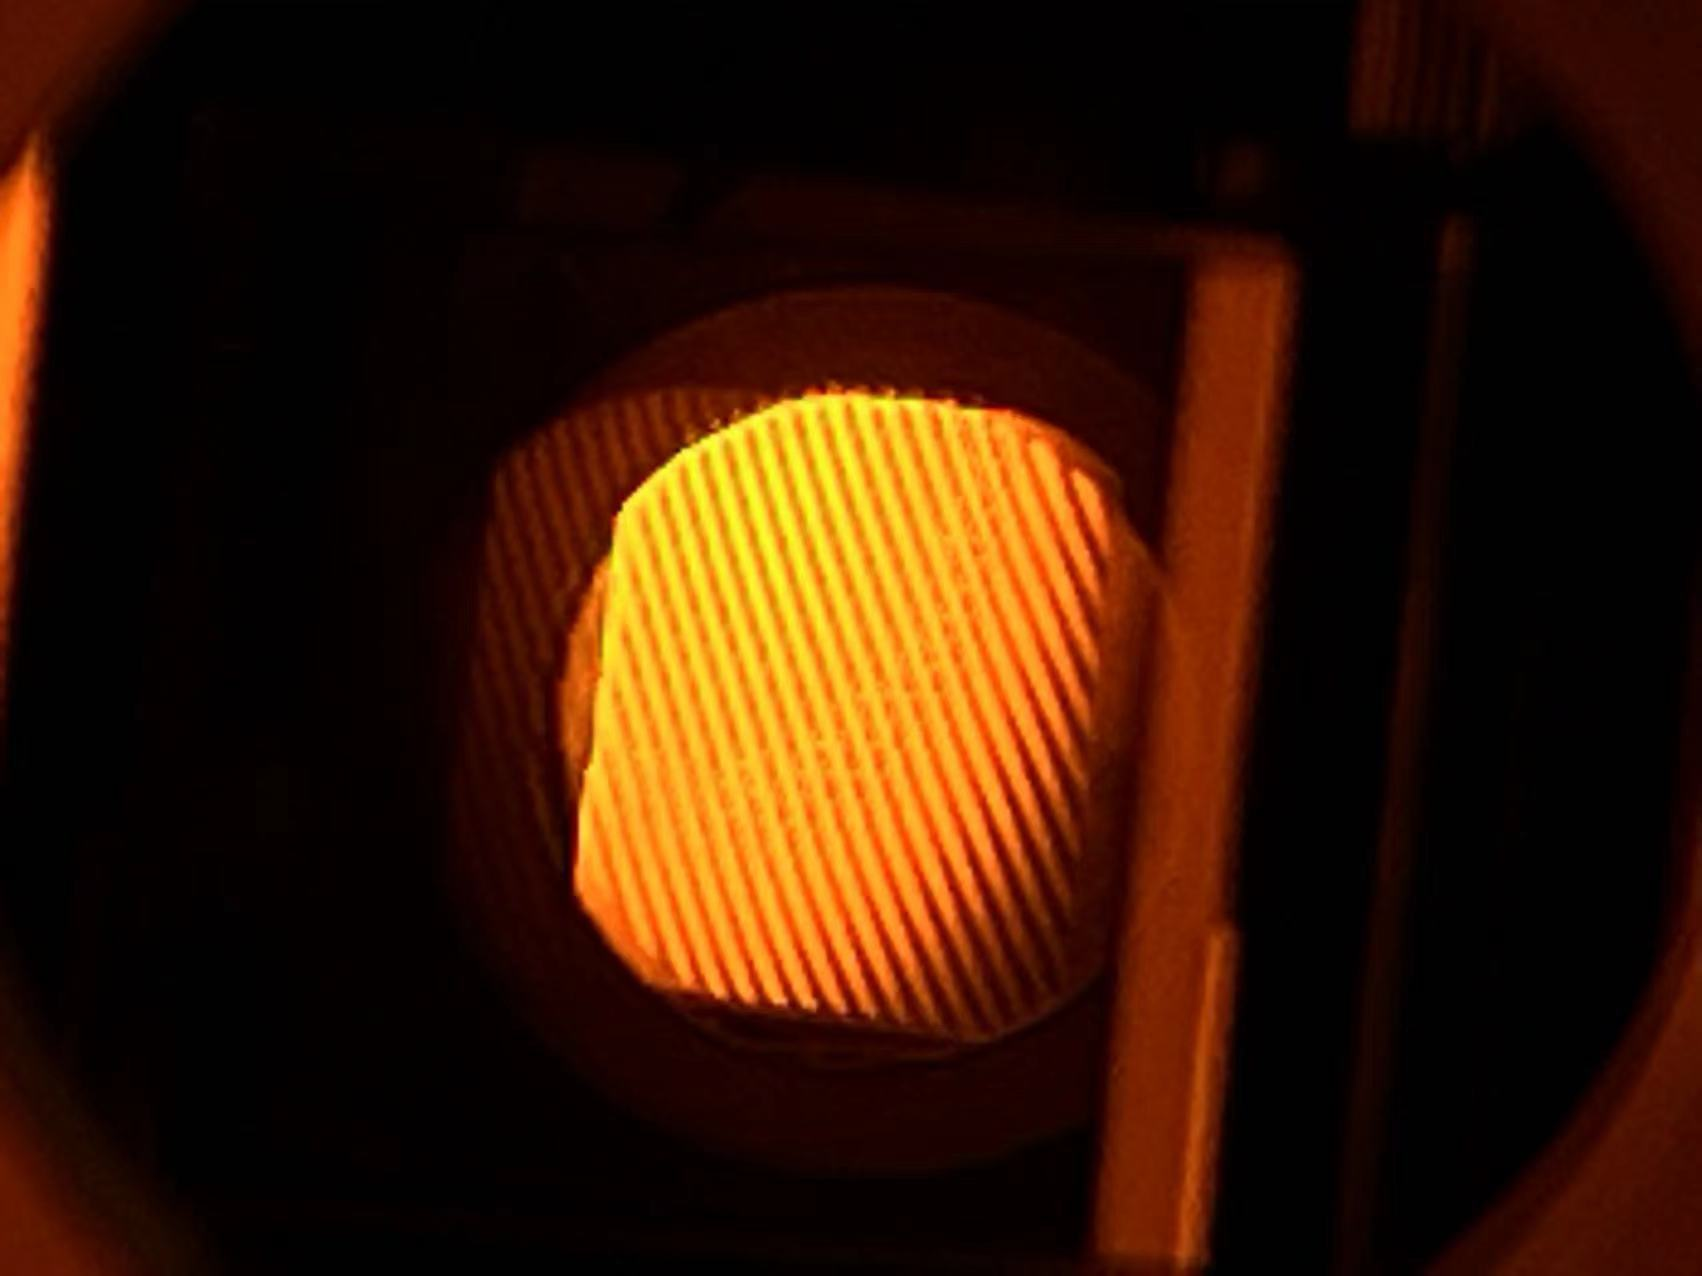
\includegraphics[width=0.7\textwidth]{graph3.jpg}
			\caption{钠黄光光源的干涉图像}
			\label{fig:graph3}
		\end{figure}
		
		实验测得的数据为:
		\[ 
		L_1=10.975mm \quad L_2=22.620mm \Longrightarrow \Delta\lambda=\frac{\bar{\lambda}^2}{2\Delta d}=\frac{(589.3\times10^{-9})^2}{2\times(\frac{(22.620-11.645)\times10^{-3}}{40})}mm=0.596nm
		 \]
		

		
		
		
		
		

	\subsubsection{实验二 白光干涉的调节,并测定透明薄片的厚度$t$或者折射率 $n$}
		
		\begin{enumerate}
			\item 用相同的方法,使用$He-Ne$激光光源调节迈克尔逊干涉仪, 使产生定域等倾干涉条纹。
			
			\item 换上扩散的白光光源(本实验中采用溴钨灯加毛玻璃代替), 微调 $M_1$精密测微头,此时应能在玻璃镜(视场)中观察到彩色的条纹,此即为“白光等厚干涉条纹”。彩色条纹之间还可观察到一条全黑的条纹,称为“中心暗纹”。
			
			\item 观察到此现象后,可缓慢调节 $M_1$ 镜的精密测微头,使中心暗纹移到视场中央,并记录下此时反射镜 $M_1$ 精密测微头的读数 $d_2$;
			
			\item 在分束镜 $P_1$ 和反射镜 $M_1$ 间安装透明薄片并与光路垂直,彩色条纹及其间的暗纹消失。缓慢调节反射镜 $M_1$ 的精密测微头(注意此时不要再调节$M_2$背面的三颗螺钉),缩小$ M_1 $和 $P_1$之间的距离,直到重新观察到彩色条纹。再缓慢调节$ M_1$ 镜,使中心暗纹移到视场中央。记录下此时反射镜 $M_1$ 精密测微头的读数$ d_1$,计算 $M_1$ 移动的距离$\Delta d = d_2 – d_1$;
			
			\item 用螺旋测微计测量薄片的厚度$ t$, 结合$\Delta d$, 根据公式计算薄片的折射率 $n=1+\frac{\lambda}{2d}$。
		\end{enumerate}
		
		\begin{figure}[htbp]
			\centering
			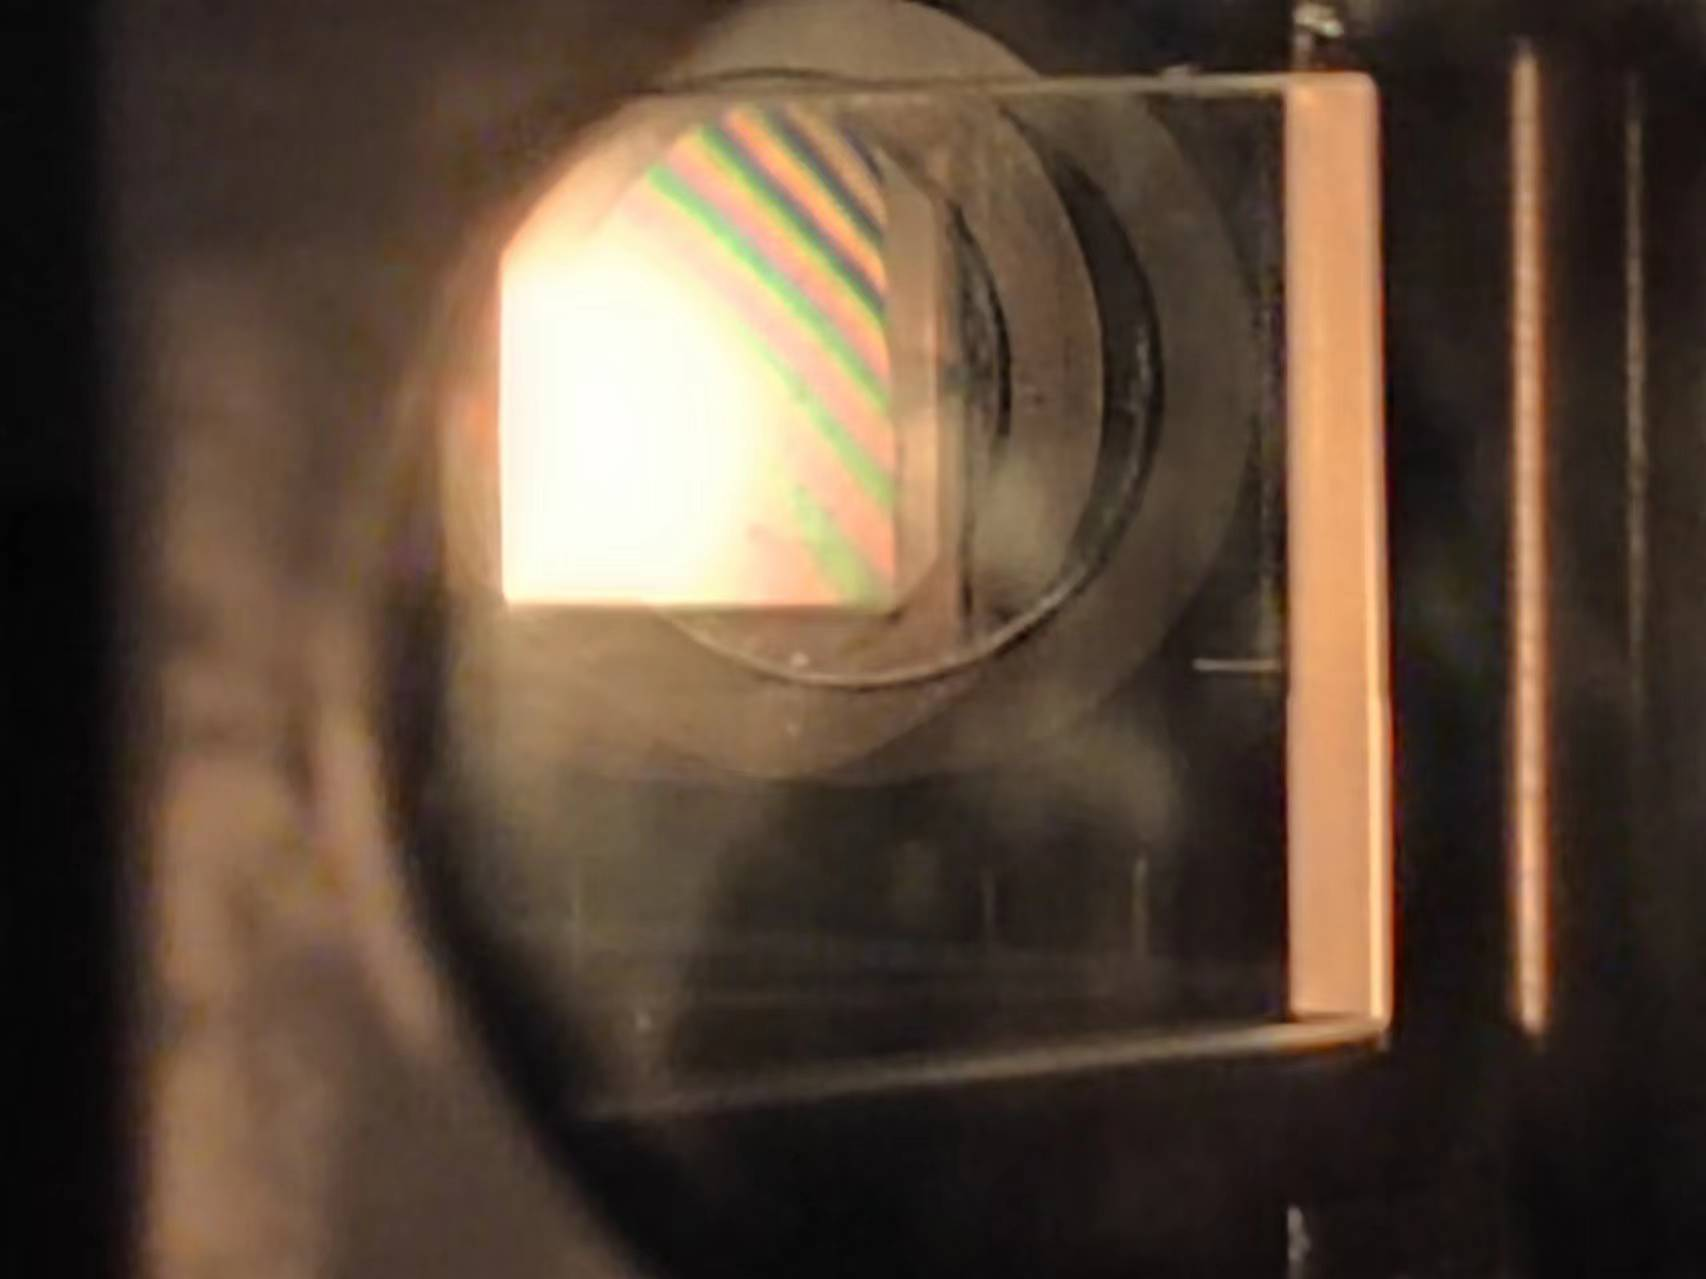
\includegraphics[width=0.7\textwidth]{graph4.jpg}
			\caption{白光光源的干涉图像}
			\label{fig:graph4}
		\end{figure}
		
		测量数据如下:
		\[ 
		L_1=16.415mm \quad L_2=13.385mm
		 \]
		\[ 
		d_0=0.910mm \quad d_1=1.085mm\Longrightarrow t=d_1-d_0=0.175mm
		 \]
		\[ 
		n=\frac{\Delta d}{t}+1=\frac{16.415-13.385}{40\times0.175}+1=1.433
		 \]
		


\subsection{实验过程中遇到的问题记录}

\begin{enumerate}
	\item 注意精密测微头存在$\frac{1}{40}$的杠杆,计算距离时要注意换算。
	
	\item 在使用$He-Ne$激光光源,使其产生定域等倾干涉条纹,然后减小两干涉臂的光程差时,一定要保持干涉圆环的圆心始终保持在视场中心,这样能保证后面调节白光干涉时成功率更高。
	
\end{enumerate}
	
	\begin{figure}[htbp]
		\centering
		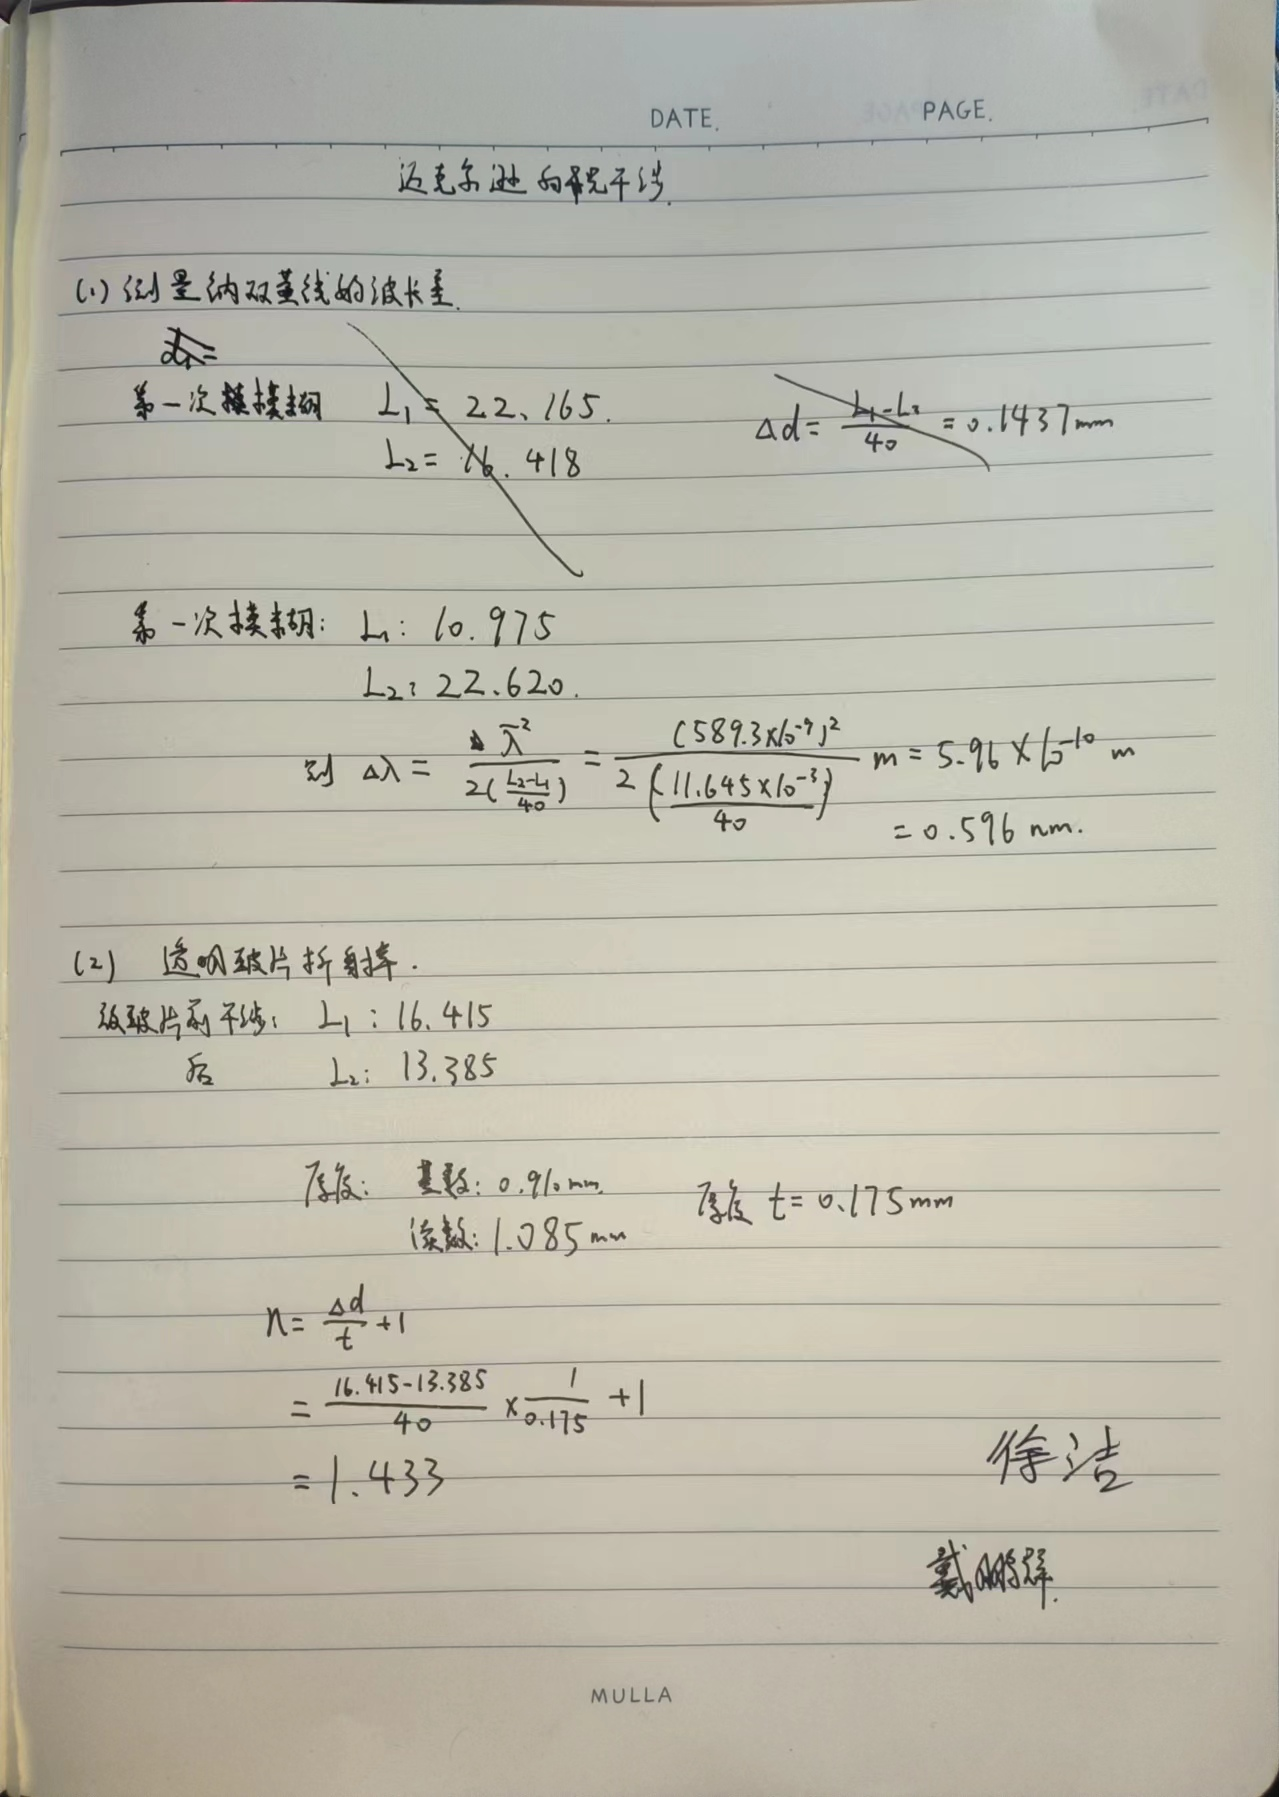
\includegraphics[width=0.7\textwidth]{ExpriData.jpg}
		\caption{实验原始数据}
		\label{fig:ExpriData}
	\end{figure}

\clearpage
\begin{table}
	\renewcommand\arraystretch{1.7}
	\begin{tabularx}{\textwidth}{|X|X|X|X|}
	\hline
	专业:& 物理学 &年级:& 2022级\\
	\hline
	姓名: & 戴鹏辉 & 学号:& 22344016\\
	\hline
    日期:& 2024/03/15 & 评分: &\\
	\hline
	\end{tabularx}
\end{table}

\section{CB1+ \quad 迈克尔逊干涉及应用(白光干涉) \quad\heiti 分析与讨论}

\subsection{实验数据分析}

	\subsubsection{实验一 测钠双黄线的波长差}
		
		
		
		
		
	\subsubsection{实验二 白光干涉的调节,并测定透明薄片的厚度$t$或者折射率 $n$}
			
			
			
			
\subsection{实验后思考题}



\begin{question}
	当空气温度变化时,空气折射率也会发生变化,请思考如何测得空气折射率。
\end{question}
	
	迈克尔逊干涉仪也可以测量空气的折射率,下面是实验方案:
	
	\begin{enumerate}
		\item 实验装置准备:准备迈克尔逊干涉仪、He-Ne激光器、气室组件、光阑、气压表和毛玻璃等。
		实验原理:迈克尔逊干涉仪利用两束相干光的干涉现象来测量光程差,从而计算出空气的折射率。当气室内的空气压强或温度变化时,会引起干涉条纹的移动,通过测量这些条纹的移动数量,可以计算出空气的折射率。
		\item 实验步骤:
		 	\begin{enumerate}[label=\roman*.]
				\item 粗调光路:确保激光束水平并且垂直入射到迈克尔逊干涉仪的反射镜$M_1$和$M_2$上。
				
				\item 细调光路:使用小孔光栏H调节光束,使之通过小孔并垂直入射在反射镜上。
				
				\item 调整干涉条纹:通过调整拉簧螺丝,使干涉条纹变粗、变疏,便于测量。
				
				\item 测量折射率:将气室抽成真空,然后缓慢充气,观察接收屏上的干涉条纹移动。记录气室内压强由0变到大气压强时的条纹变化数,利用公式计算空气的折射率。
			\end{enumerate}

		\item 数据处理:收集多组数据,计算平均值,以提高实验的准确性。
		 
		\item 注意事项:
			\begin{enumerate}[label=\roman*.]
				\item 避免直接触摸光学表面。
				\item 实验中应保持安静,避免走动影响实验结果。
				\item 注意激光安全,避免直视激光束。
			\end{enumerate}
	\end{enumerate}
	
	通过上述实验方案,可测量出空气的折射率。我们可以用这样的方法,记录下不同温度下,空气的折射率,并由此绘制出关系曲线,分析空气折射率与温度的关系。

	
	
	
	
	\begin{figure}[htbp]
		\centering
		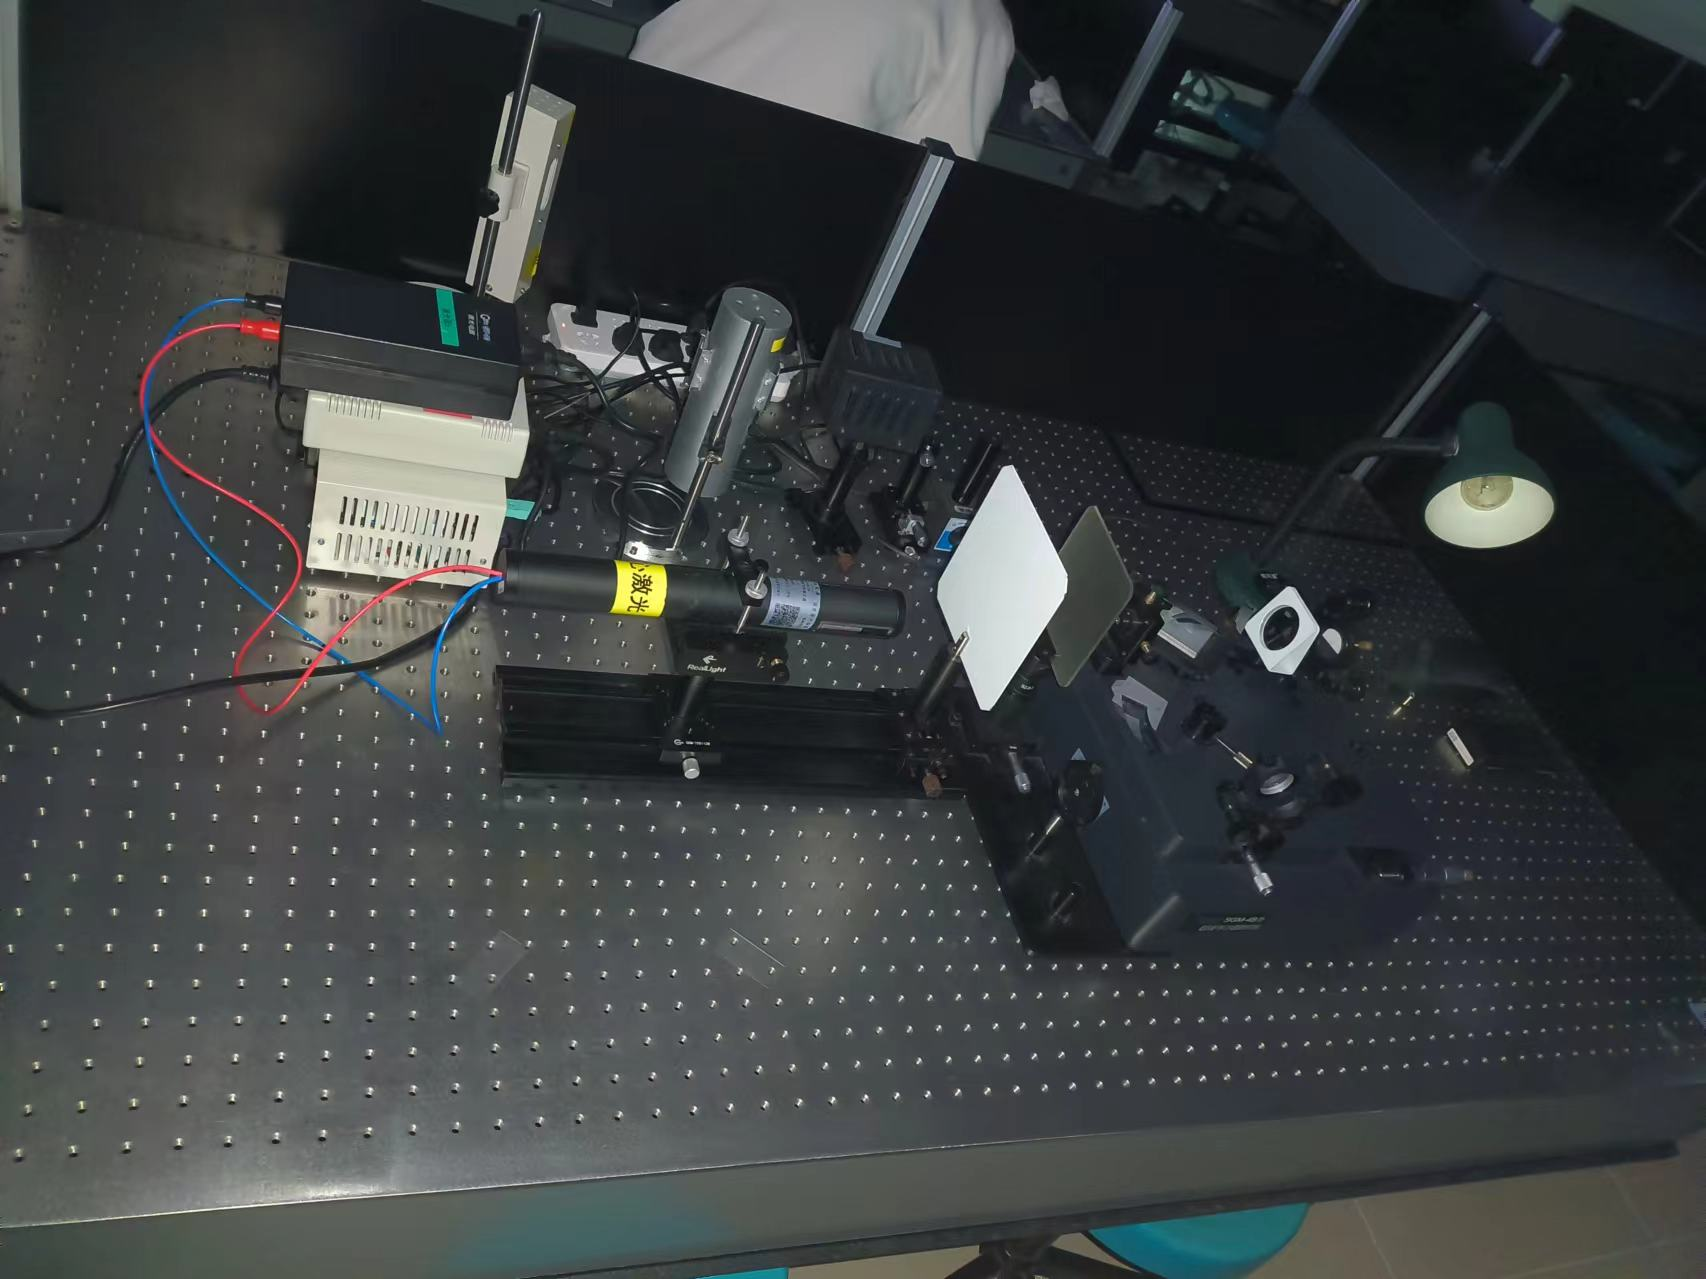
\includegraphics[width=0.7\textwidth]{table.jpg}
		\caption{整理后实验桌照片}
		\label{fig:table}
	\end{figure}
	

\end{document}
